% Chapter Template

\chapter{TLA\textsuperscript{+}} % Main chapter title

\label{TLA+} % Change X to a consecutive number; for referencing this chapter elsewhere, use \ref{ChapterX}

We specify a system as a set of possible behaviours representing a correct execution
of the system. We define a behaviour as a sequence of states. A state is defined
as an assignment of values to variables. 

\begin{figure}[H]
	\centering
	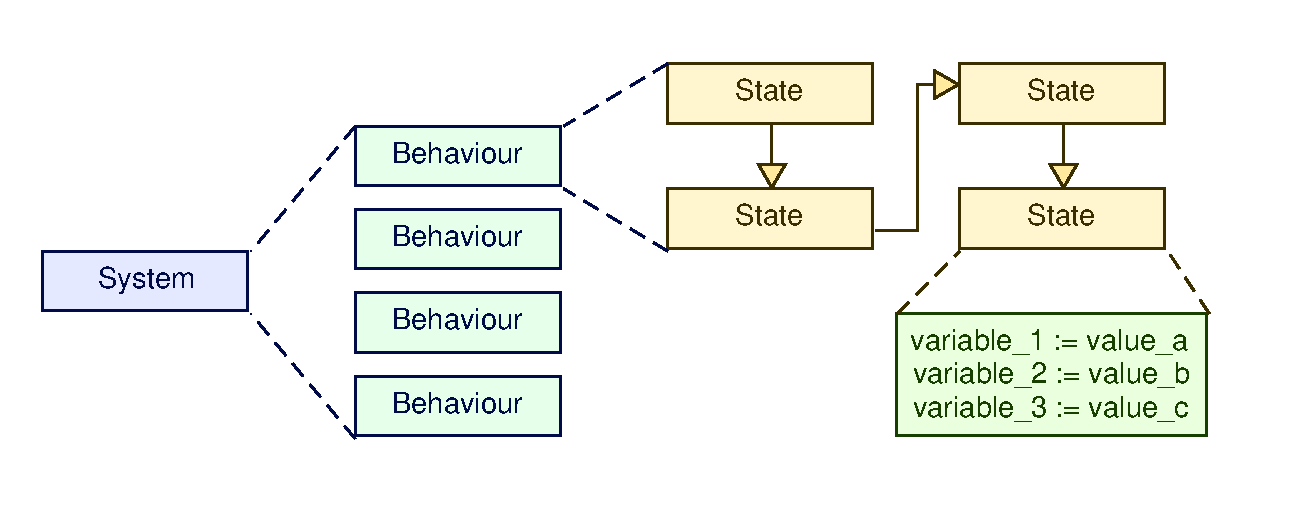
\includegraphics[scale=0.75]{Figures/System_Specification.pdf}
	\decoRule
	\caption{System specification.}
	\label{fig:SysSpec}
\end{figure}

\section{Writing a Specification}

\subsection{Boilerplate}
System are specified in module files. You should use the module name for the file name with a .tla extension.

\begin{lstlisting}[language = TLA, literate={-}{{-\allowbreak}}{1}]
------------------------- MODULE module_name ------------------------
EXTENDS \*  list modules
VARIABLES \* list variables
\* system specification
---------------------------------------------------------------------

=====================================================================
\end{lstlisting}

\subsection{Variables, Type Invariant, Initial Predicate}

Decide what variables you are going to use to describe your system. It is usually
better to use high-level, abstract descriptions of the system’s data structures
in a specification.

TLA\textsuperscript{+} only has four basic kinds of values: strings, integers, 
booleans, and model values[]. To create more intresting types we 

\subsection{Next-State Action}
First, pick the variables and define the type invariant and initial predicate.
	
\subsection{Temporal specification}	

\section{Info}

\begin{description}
	\item [state function] An ordinary expression (one with no prime or \( \Box \) ) that can contain variables and constants.
	\item [state predicate] A Boolean-valued state function.
\end{description}

\begin{description}
	\item [safety properties] 	Specify valid behaviour. Specify what is allowed to happen. If a safety property is 
						violated, it is violated at a specific point in the behaviour. If a safety 
						property has been satisfied it means the safety property has not been
						violated by any step in the behaviour so far.
	\item [liveness properties]	Specify what behaviour that cannot be violated at any particular instant.
\end{description}

Formally a temporal formula F assigns a Boolean value, which we write \(  \sigma \vDash F \), to a behaviour \( \sigma \).
We say that F is true of \( \sigma \), or that \( \sigma \) satisfies F, iff \( \sigma \vDash F \) equals TRUE.

\begin{enumerate}
	\item  A state predicate, viewed as a temporal formula, is true of a behaviour iff it is true in the first state of the behaviour.
	\item  A formula \( \Box P \), where \(P\) is a state predicate, is true of a behaviour iff \( P \) is true in every state of the behaviour.
	\item  A formula \( \Box[N]_{v} \), where N is an action and \(v\) is a state function, is true of a behaviour iff 
		every successive pair of steps in the behaviour is a \( [N]_v \) step.
\end{enumerate}


\begin{description}
	\item [\( \Diamond \) F ] It asserts that F is not always false, which means that F is true at some time.
		We usually read \( \Diamond \) as eventually, taking eventually to include now.
	\item [ \( F \leadsto G \) ] asserts that whenever F is true, G is eventually true.
		We read \( \leadsto \) as leads to.
	\item [\(  \Diamond \langle A \rangle_v \) ] asserts that eventually an \( \langle A \rangle_v \) step occurs
	\item [ \( \Box \Diamond F \) ] asserts that at all times, F is true then or at some later time.
		In particular,\( \Box \Diamond \langle A \rangle_v \) asserts that infinitely many \( \langle A \rangle_v \) steps occur.
	\item [ \( \Diamond \Box F \) ] asserts that eventually (at some time), F becomes true and remains true thereafter.
		\( \Diamond \Box [N]_v \) asserts that, eventually, every step is a \([N]_v\) step.
\end{description}



\section{How to structure a document}

\section{basics}

\section{Verify}